
\section*{2. Implementation}

%----------This part will give a a short intro to implementation and will flow into pre-processing subsection.

In this section, we explain all aspects of our implementation, starting with the characteristics of the input data set, how we perform pre-processing, then tokenize the data. We then give details about the implementation of our Recurrent Neural Net, and how we train it.

\subsection*{2.1 Data set characteristics}
%-----give details about the data set, lead to preprocessing

The input data set has the format as shown in Figure \ref{input}. The input file was formatted as a comma-separated values (".csv") file, where the different fields are separated by commas. 

\begin{figure}[h]
\centering
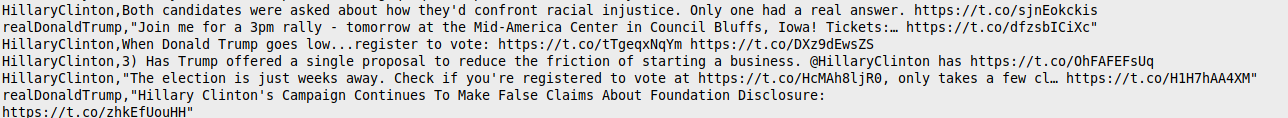
\includegraphics[scale=.36]{inputs.png}
\caption{This image shows the format of the input file.} \label{input}
\end{figure}

The first field is the Twitter handle of the candidate, which serves as the label for the tweet, HillaryClinton (Hillary Clinton), realDonaldTrump (Donald Trump). The second field contains the tweet. There were a total of 4743 tweets in the input data set.

The test data set was given in the same format, ie. a .csv file, containing a total of 1701 tweets, but had the handle replaced with "none". 

	As we could not validate our predictions due to the absence of labels in the test data set, the results needed to be submitted to kaggle, as a .csv file, formatted as shown in Figure \ref{format}, to be compared against other groups.

\begin{figure}[h]
\centering
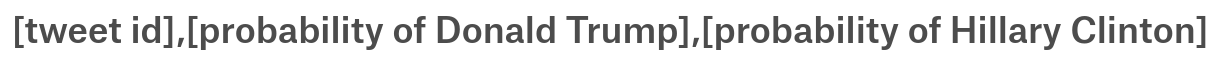
\includegraphics[scale=.35]{format.png}
\caption{Submission Format} \label{format}
\end{figure}	

The next section provides more information about the preprocessing that was performed on the dataset. 

